\section{Durchführung}
\label{sec:Durchführung}
\subsection{Lasergranulation}
\label{sec:Lasergranulation}
Um den Schwellenstrom zwischen LED (light emitting diode) und Laserlicht zu bestimmen,
wird der Effekt der Lasergranulation verwendet.
Lasergranulation tritt auf, wenn Laserlicht auf eine unebene Fläche trifft 
und dort reflektiert wird.
Nach dem Huygen'schen Prinzip entsteht dabei an jeder Unebenheit eine neue Kugelwelle.
Trift nun monochromatisches Licht auf diese Streuzentren entsteht ein zufälliges Interferenzmuster,
welches als körnige Lichtflecke zu erkennen sind.
Um diesen Schwellenstrom zu bestimmen, wird eine unebene Oberfläche in den Laserstrahl gebracht (vgl. Abbildung \ref{fig:Lasergranulation}).
\begin{figure}[h]
    \centering
    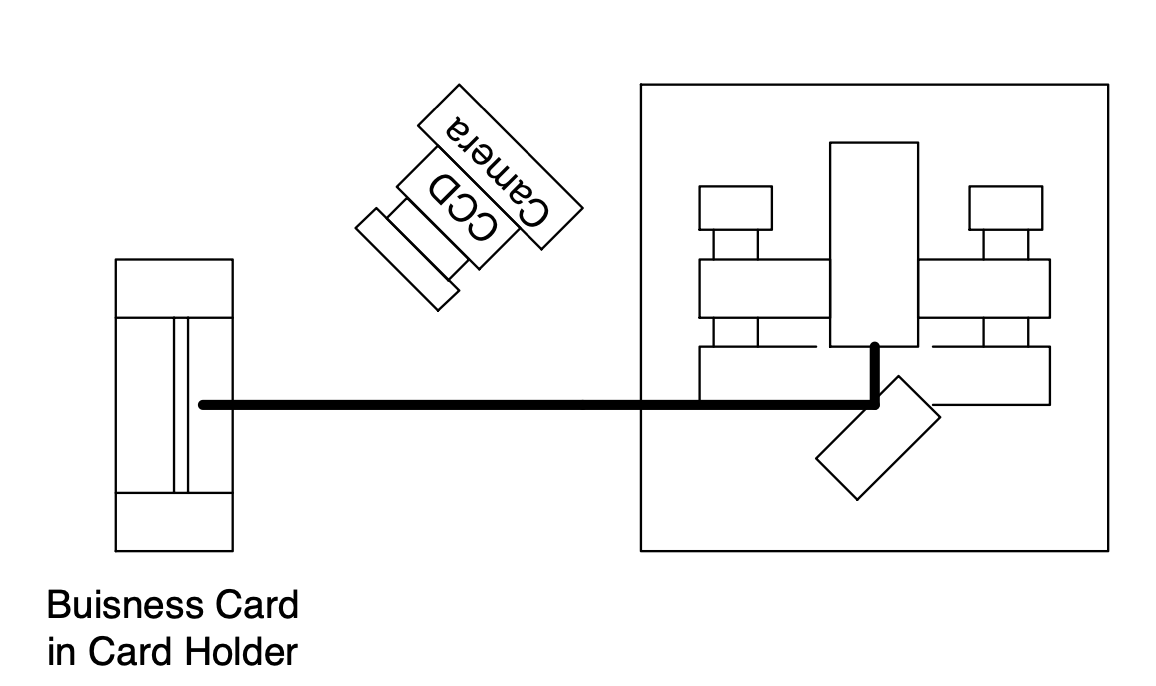
\includegraphics[width=0.7\textwidth]{abb/aufbau1.png}
    \caption{Aufbau Lasergranulation \cite{aufbau}}
    \label{fig:Lasergranulation}
\end{figure}
Strom und Winkel des Lasers werden so eingestellt,
dass Lasergranulation beim kleinstmöglichen Strom auftritt.
Die CCD Kamera dient als Detektor für das Infrarotlicht,
da dieses mit bloßem Auge nicht zu erkennen ist.

\subsection{Aufnahme des Transmissionsspektrums von Rubidium}
Im nächsten Schritt wird der Laser, 
wie in Abbildung \ref{fig:Rub},
durch eine Rubidium Zelle gelenkt.
\begin{figure}
    \centering
    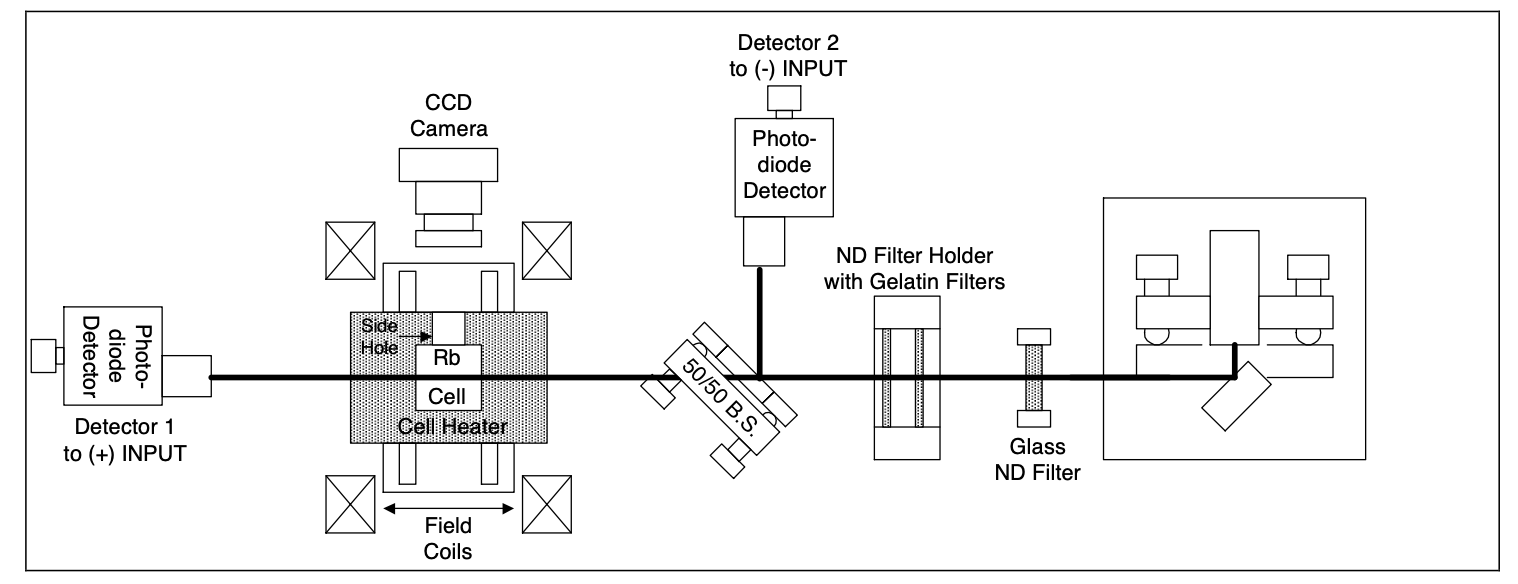
\includegraphics[width=0.7\textwidth]{abb/rub.png}
    \caption{Aufbau zum Ermitteln der Emissionslinien von Rubidium \cite{aufbau}}
    \label{fig:Rub}
\end{figure}
Die CCD-Kamera wird Richtung Rubidium Zelle ausgerichtet,
um ein optisches Feedback zu erlangen.
Zunächst wird ohne die Filter und den $50/50$-Strahlteiler der Laser so eingestellt,
dass in der Rubidium Zelle Ionisierung auftritt.
Zu erkennen ist dies durch einen Lichtstrahl auf dem Bildschirm der CCD-Kamera.
Zur Einstellung stehen neben dem optischen Gitter ebenfalls ein Piezo-Kristall,
der sein Volumen abhängig von der Stromstärke ändert.
Der Kristall bietet den Vorteil einer genaueren Justierung, 
als mit dem Gitter.
Anschließend werden der Strahlteiler und die Filter dem Versuchsaufbau hinzugefügt.
Der Strahlteiler und der zweite Detektor dienen dazu, den Hintergrund herauszufiltern.
Die Filter werden eingebaut, um die Fotodiode zu schonen.
Wichtig ist bei der Arbeit mit den Fotodioden, 
dass der Raum abgedunkelt ist,
um die Messung nicht zu verfälschen.
Der Aufbau ist nun so zu justieren,
dass im gemessenen Spektrum keine Mode Hops mehr auftreten.
Diese erkennt man an plötzlich abfallender Lichtintensität im Messgraphen.
Treten Mode Hops auf, können die verschiedenen Peaks nicht mehr eindeutig zugeordnet werden.